\documentclass{article}
\usepackage[utf8]{inputenc}
\usepackage{amsmath}
\usepackage{listings}
\usepackage{geometry}
\usepackage{graphicx}
\usepackage{appendix}
\usepackage{subfig}
\usepackage{subcaption}
\usepackage{gensymb}
\usepackage{cancel}
\usepackage{physics}
\usepackage[colorlinks=true]{hyperref}
\usepackage{xcolor}
\definecolor{codegreen}{rgb}{0,0.6,0}
\definecolor{codegray}{rgb}{0.5,0.5,0.5}
\definecolor{codepurple}{rgb}{0.58,0,0.82}
\definecolor{backcolour}{rgb}{0.95,0.95,0.92}
\lstdefinestyle{mystyle}{
    backgroundcolor=\color{backcolour},   
    commentstyle=\color{codegreen},
    keywordstyle=\color{magenta},
    numberstyle=\tiny\color{codegray},
    stringstyle=\color{codepurple},
    basicstyle=\ttfamily\footnotesize,
    breakatwhitespace=false,         
    breaklines=true,                 
    captionpos=b,                    
    keepspaces=true,                 
    numbers=left,                    
    numbersep=5pt,                  
    showspaces=false,                
    showstringspaces=false,
    showtabs=false,                  
    tabsize=2
}

\lstset{style=mystyle}

\title{%
Comparing and Studying Neural Network Models \\
using a Double Pendulum System \\
\large FYS5429 at University of Oslo}
\author{Simen Løken}
\date{May 2023}
\footskip = 90pt
\topmargin = -40pt

\begin{document}
\nocite{*}
\maketitle
{
  \hypersetup{linkcolor=black}
  \tableofcontents
}\newpage
\section{Abstract}
The double pendulum system is an iteresting system in physics given its chaotic behavior. In this project we will study such a system using various different Neural Network models and weighing them against each other. We will be using a Feed Forward Neural Network, a Recurrent Neural Network and a Convolutional Neural Network. To do this we will first study how to numerically generate sufficient double pendulum data using a Runge-Kutta 4 method, then compare the models. Ultimately, the models are very close, but we find that Convolutional Neural Networks are surprisingly effective in their modelling of such systems.
\section{Introduction}
When studying a system like a double pendulum, one of the most common ways to solve and study them is through the use of numerical methods like the Euler Method or the Runge-Kutta family of methods. Typically, one would take some initial variables and use them, with some suitable timestep, to predict how the system would unfold as time progresses. This is all well, but still somewhat limited. In this project, we're going to look at an alternative method of studying such numerical systems, namely by using Neural Networks \newline
Neural Networks are deceptively good at handling and solving numerical systems. As opposed to traditional numerical methods, Neural Networks can solve systems without underlying explicit mathematical models or equations. That is, it can learn the system purely through data. This is called a data-driven approach to numerical modelling, and allows us to even model systems too complex or without sufficient domain knowledge. \newline
Additionally to this, Neural Networks are often more stable than their numerical counterparts. With a problem like double pendulums, you'll often find that even small changes to the initial variables can have explosive results, and some times the simulation will break. This is highly unlikely with Neural Networks. As Neural Networks are trained on a large amount of data, it is rare, if not impossible for a well trained Neural Network to predict a "broken" simulation for a given set of initial variables.\newline
It are these (and more) attributes that make Neural Networks a very interesting field within the computational sciences, and in this project we're going to study from the ground up how you can create a suitable Neural Network to study a rather chaotic system like that of double pendulums.
\section{Theory and Method}
\subsection{Neural Networks - What are they?}
Neural Networks are inspired by our brains in the way they are made. At their simplest, a Neural Network consist of an input layer, hidden layer(s) and an output layer. Input layers receive what we put into the Neural Network. It is then passed onto the neurons (hence the name) which is the hidden layer. Each neuron in the hidden layer has a set of weights and biases, which in turn determine the connections between the neurons and the sensitivity to input. The weights and biases are updated as the network trains. After being passed through all the hidden layers, we get an output. \newline
\subsubsection{Feed-Forward Neural Network}
The simplest form of the Neural Network, the Feed-Forward Neural Network (FFNN) is named as such because the information flows forward. That is, information only ever flows from the input layer to the output layer. It never experiences any recurrent connections.
\newline Although they are simple, that is not to say they are weak. Even just a shallow FFNN can be more than sufficient for many computational tasks.
\subsubsection{Recurrent Neural Network}
Perhaps the most relevant to what we're going to be exploring, Recurrent Neural Networks (RNN) is a Neural Network that is designed to handle sequential data. That is to say, the order of the inputs matter. This, in turn, makes it very suitable for solving time-sensitive numerical systems, such as the double pendulum system we're going to be examining. \newline
RNNs, as the name suggests, has recurrent connections. Whereas in a FFNN, a given neuron only recieves information from a previous layer, a neuron in an RNN also recieves information from its previous state. In turn, this allows a given neuron to retain a sort of pseudo-memory or context. \newline
There are many different types of RNN, but we're specifically going to be using a Long Short-Term Memory (LSTM) network. RNNs inherently have a problem where the gradients used to update the weights diminish exponentially as they propogate (either through layers or time steps), which in turn weakens the pseudo-memory of a given neuron and leads to poor learning. An LTSM model combats this by further expanding on the memory of an RNN, as LTSMs can selectively retain or forget information. This is done through introducing "gates" to each portion of the neural network. An input gate, a hidden(or forget) gate and a output gate, where the input gate determines how much of the input will be stored, the hidden gate determines which parts of the previous state to forget and the output gate which regulates the information recieved from the input and hidden gate. This in turn allows for a very powerful model.
\subsubsection{Convolutional Neural Network}
Lastly we're going to be using Convolutional Neural Networks (CNN). Typically, CNNs are used to study or model images and video, which may raise some eyebrows as to why we're using this here. However, if we assume we have an input of some $x$ timesteps worth of 2d data, length $y$, such that the shape is $(y, x, 2)$. A given input is then of shape $(x,2)$, and we can reshape it to be $(x, 2, 1)$. This in turn, effectively allows us to model our data as if it was an image, which is what CNNs are made for.
\newline
As hinted at above, CNNs are uniquely good at images and video, or to be more accurate, grid-like data, which may be more of an explanation as to why we're rearranging our data to be a grid. As to why CNNs are so useful with grid-like data, a CNN has three types of layers. Firstly, there are convolutional layers (hence the name). Secondly there are pooling layers and lastly the fully connected layers. Convolutional layers are a set of learnable filters that perform convolutional operations on the input data. this is done by letting the filters scan the input and extract local patterns. The pooling layers reduce the spacial dimensions of the data while retaining important features. This is important, as CNNs are very computationally heavy compared to the other Neural Networks in this project. Lastly, the connected layers are similar to those in normal FFNN and have the final say before it reaches the output layer, that is to say, the connected layers produce the output through aggregated extracted features from the previous layers. \newpage
\subsection{Data Generation}
As we need data to train our Neural Network, we will be using a Runge-Kutta4 numerical method to generate the data. The Runge-Kutta4 is a well known and popular method, but for simplicity's sake, let us go through it:
\begin{equation}
    y_{n+1} = y_n + \frac{h}{6} \sum_{i=1}^4 b_i k_i = y_n + \frac{h}{6} \left(k_1 + 2k_2 + 2k_3 + k_4\right)
\end{equation}
where:
\begin{equation*}
    k_1 = h f(x_n, y_n)
\end{equation*}
\begin{equation*}
    k_2 = h f\left(x_n + \frac{h}{2}, y_n + \frac{k_1}{2}\right)
\end{equation*}
\begin{equation*}
    k_3 = hf(\left(x_n + h, y_n + \frac{k_2}{2}\right)
\end{equation*}
\begin{equation*}
    k_4 = hf(x_n + h, y_n + k_3)
\end{equation*}
where $h$ is the timestep.
\subsubsection{Double Pendulums - Numerically}
We also need to find the appropriate solution to the Double Pendulum system, numerically. First, we must find the Lagrangian $L$:
\begin{equation*}
    L = T-V = T_1 + T_2 - (V_1 + V_2)
\end{equation*}
where
\begin{equation*}
    T_1 = \frac{1}{2} M_1 \left(\dot x_1^2 + \dot y_1^2\right)
\end{equation*}
\begin{equation*}
    T_2 = \frac{1}{2} M_2 \left(\dot x_2^2 + \dot y_2^2 \right)
\end{equation*}
and
\begin{equation*}
    V_1 = gM_1y_1 
\end{equation*}
\begin{equation*}
    V_2 = g M_2 y_2
\end{equation*}
Using then that $x$ and $y$ for pendulum 1 and 2 is expressed as:
\begin{equation*}
    x_1  = L_1 \sin(\theta_1)
\end{equation*}
\begin{equation*}
    y_1 = -L_1 \cos(\theta_1)
\end{equation*}
\begin{equation*}
    x_2 = x_1 + L_2 \sin(\theta_2)
\end{equation*}
\begin{equation*}
    y_2 = y_1 - L_2 \cos(\theta_2)
\end{equation*}
The Lagrangian then becomes:
\begin{equation*}
\begin{aligned}
L &= \frac{1}{2} (M_1 + M_2) L_1^2 \dot{\theta_1}^2 + \frac{1}{2} M_2 L_2^2 \dot{\theta_2}^2 \\
&\quad+ M_2 L_1 L_2 \dot{\theta_1} \dot{\theta_2} \cos(\theta_1 - \theta_2) \\
&\quad+ (M_1 + M_2) g L_1 \cos(\theta_1) + M_2 g L_2 \cos(\theta_2)
\end{aligned}
\end{equation*}
Solving then:
\begin{equation*}
    \frac{d}{dt} \left( \frac{\delta L}{\delta \dot \theta_1}\right) - \frac{\delta L}{\delta \theta_1} = 0
\end{equation*}
\begin{equation*}
    \frac{d}{dt} \left( \frac{\delta L}{\delta \dot \theta_2}\right) - \frac{\delta L}{\delta \theta_2} = 0
\end{equation*}
We find the accelerations:
\begin{equation}
\ddot \theta = \alpha_1 = \frac{{-g(2M_1+M_2)\sin(\theta_1) - M_2g\sin(\theta_1-2\theta_2) - 2\sin(\theta_1-\theta_2)M_2(\omega_2^2L_2+\omega_1^2L_1\cos(\theta_1-\theta_2))}}{{L_1(2M_1+M_2-M_2\cos(2\theta_1-2\theta_2))}}
\end{equation}
\begin{equation}
\ddot \theta = \alpha_2 = \frac{{2\sin(\theta_1-\theta_2)(\omega_1^2L_1(M_1+M_2) + g(M_1+M_2)\cos(\theta_1) + \omega_2^2L_2M_2\cos(\theta_1-\theta_2))}}{{L_2(2M_1+M_2-M_2\cos(2\theta_1-2\theta_2))}}
\end{equation}
\newline
We can imagine such a system to look like this:
\begin{figure}[ht!]
    \centering
    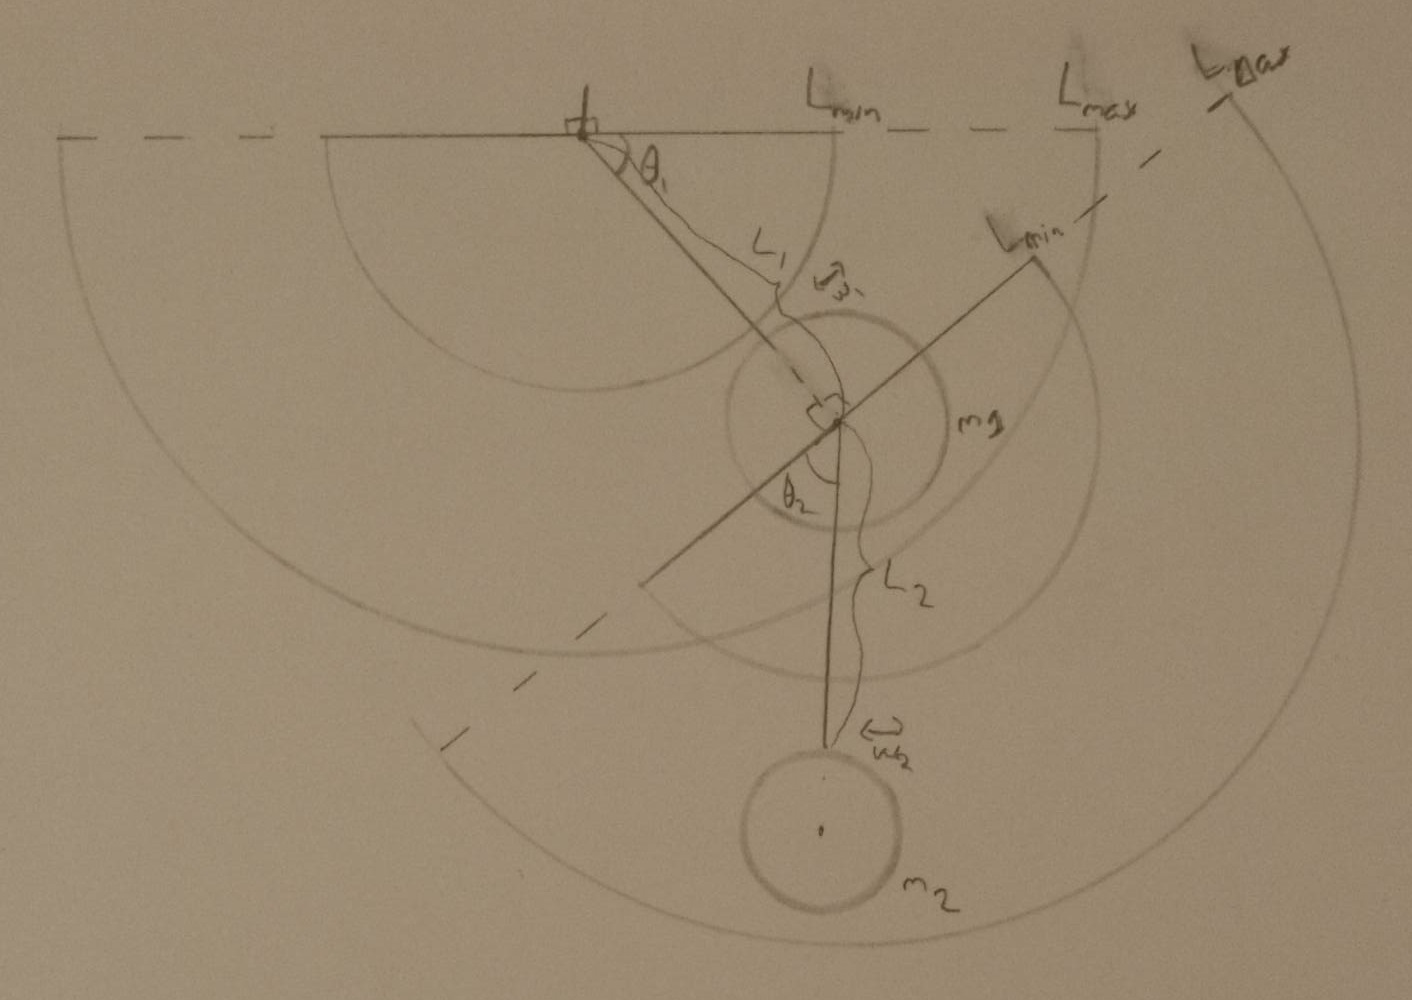
\includegraphics[scale=0.25]{systemDrawing.jpg}
    \caption{One possible configuration of our system \newline We have a first pendulum 1, whose length $L_1$ lies within $L_{min}$ and $L_{max}$ the possible values $\theta_1$ lie within the $\theta_{min}$ and $\theta_{max}$ in relation to the vertical. Additionally, $\omega_1$ and $m_1$ are also randomized within the boundaries of $\omega_{min}, \omega_{max}$ and $\m_{min}, m_{max}$ \newline Similarly, pendulum 2 also uses the same limits, but its angle $\theta_2$ is instead relative to the angle $\theta_1$, essentially making its limits $\theta_1 + \theta_{min}$ and $\theta_1 + \theta_{max}$}
    \label{figEx}
\end{figure} \newline
where the limits are:
\begin{table}[ht!]
    \centering
    \begin{tabular}{c|c|c|c|c}
          &L [m]& $\theta$ [rad]& $\omega$ [m/s] & m [kg]  \\
          \hline
         $_{min}$& $0.5$& $-\frac{\pi}{2}$& $-0.05$& $0.25$ \\
         $_{max}$& $1$& $\frac{\pi}{2}$& $0.05$& $0.5$
    \end{tabular}
    \caption{The limits we define for the randomized initial variables for our system.}
    \label{tabEx}
\end{table}
\newpage
\section{Results}
First, we implement our RK4 model to generate a sufficient data set for us to use. To ensure a sufficiently accurate model, we create a heat map for pendulum 2, with a total of 1000 runs. \newline We find:
\begin{figure}[ht!]
    \centering
    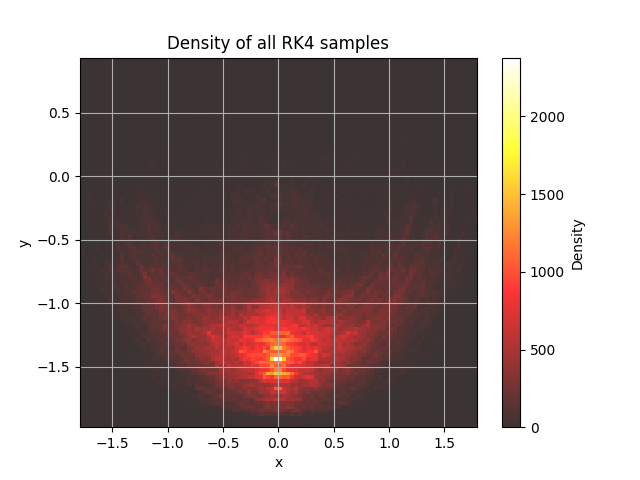
\includegraphics[scale=0.45]{RK4_density.png}
    \caption{A heat map of all positions $x_2, y_2$ over a period of 5 seconds. As predicted, it takes the shape of an $\omega$ or a $w$. It may at first be odd that we do not see a crescent shape, but this is because occasionally pendulum 2 will pivot about pendulum 1 as it normally along the "bottom" of its path. This behavior can be seen easier in Fig. [\ref{figRK4T}]}
    \label{figRK4D}
\end{figure} \newline
To doubly study this movement, we take a small subsection of all samples and plot the path traced by pendulum 2. \newline We get:
\begin{figure}[ht!]
    \centering
    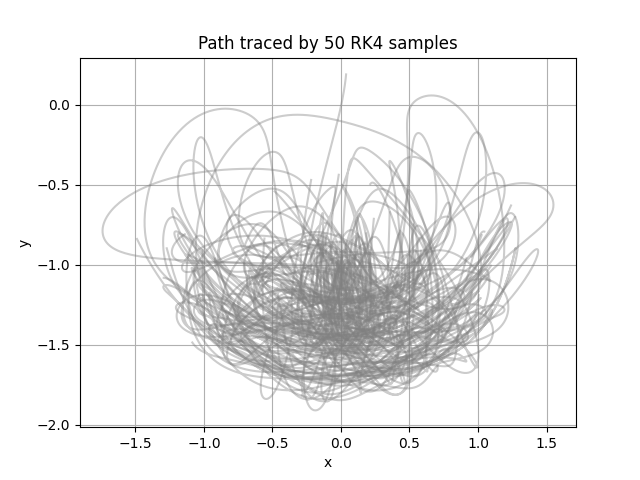
\includegraphics[scale=0.45]{RK4_50traced.png}
    \caption{The path traced by 50 pendulum 2's over a period of 5 seconds. As mentioned above we see here the somewhat characteristic $\omega$ or $w$ movement.}
    \label{figRK4T}
\end{figure}
\newpage 
Let use now examine the three different Neural Networks we will be using head to head.
\begin{figure}[ht!]
    \centering
    
    \begin{minipage}{0.48\textwidth}
        \centering
        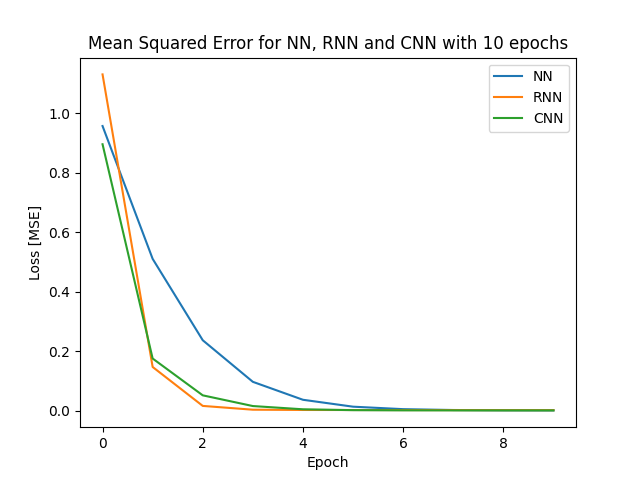
\includegraphics[scale=0.4]{training_error_macro.png}
        \caption{A macro image of the training error}
        \label{fig:macro_error}
    \end{minipage}\hfill
    \begin{minipage}{0.48\textwidth}
        \centering
        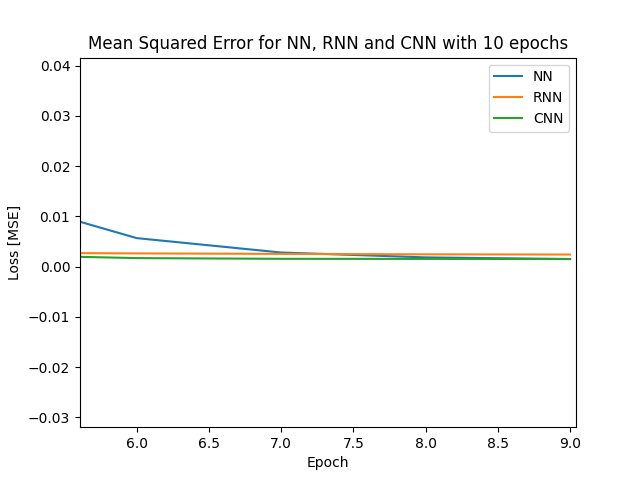
\includegraphics[scale=0.4]{training_error_micro.png}
        \caption{A micro image of the training error}
        \label{fig:micro_error}
    \end{minipage}
    \caption{A macro and micro image of the training errors for the different models over 10 epochs. We see here, perhaps somewhat surprisingly, that NN and CNN outperforms RNN, but only slightly. \newline
    As for the test losses for this run, we get:
    \newline NN: $0.517 \;\;\;$ RNN: $0.529 \;\;\;$ CNN: $0.571$ \newline} 
    \label{fig:training_errors}
\end{figure}
\newline
The fact that, relatively, CNN performs much worse (again, relatively) than RNN and NN in terms of test error, could be indicative of some kind of overfitting.
We move now on to doing the simulations with the models. As it is hard to gauge the success rate of a model purely from the training and test error. It can give us a good benchmark, but to truly see if our model is good, we must compare it to the real deal. \newpage
To do this, we will create plots similar to those found in Fig. [\ref{figRK4D}] and Fig. [\ref{figRK4T}], but for each of the different models. 
Starting first with NN:
\begin{figure}[ht!]
    \centering
    
    \begin{minipage}{0.48\textwidth}
        \centering
        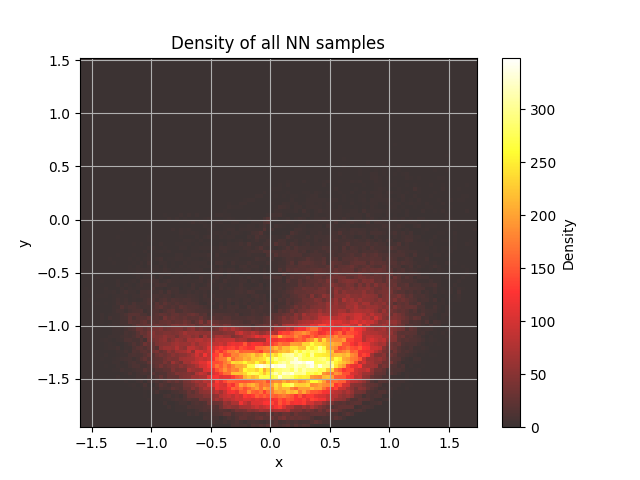
\includegraphics[scale=0.4]{NN_density.png}
        \caption{A heat map of pendulum 2 in the predicted NN model}
        \label{figNND}
    \end{minipage}\hfill
    \begin{minipage}{0.48\textwidth}
        \centering
        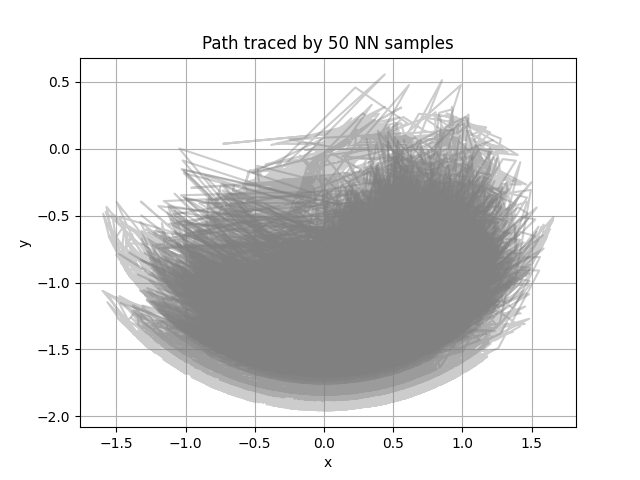
\includegraphics[scale=0.4]{NN_50traced.png}
        \caption{50 samples of pendulum 2 traced with the NN model}
        \label{figNNT}
    \end{minipage}

    \caption{We see here the a heat map and 50 traced samples respectively. At face value, it's easier to extract data from Fig. [\ref{figNND}] than Fig. [\ref{figNNT}]. We see that the model somewhat understands what an oscillation is when averaged out, but looking at the density bar, we see that its peak value is much, much lower than that of Fig. [\ref{figRK4D}]. This suggests that although the model somewhat understands, it is much more random in its prediction than it's "real" counterpart. As for the other image, we see here clearly that the movement of pendulum 2 is much more random than in the RK4 simulation. \newline
    \textit{It is worth noting that the RK4 heat map is 1000 simulations. This heat map (and subsequent ones) are 200. Thus, the density is expected to be lower, but not by this much (if equal, this density bar should've peaked at atleast 400)}}
    \label{figNN}
\end{figure}

\newpage
Next is RNN:
\begin{figure}[ht!]
    \centering
    
    \begin{minipage}{0.48\textwidth}
        \centering
        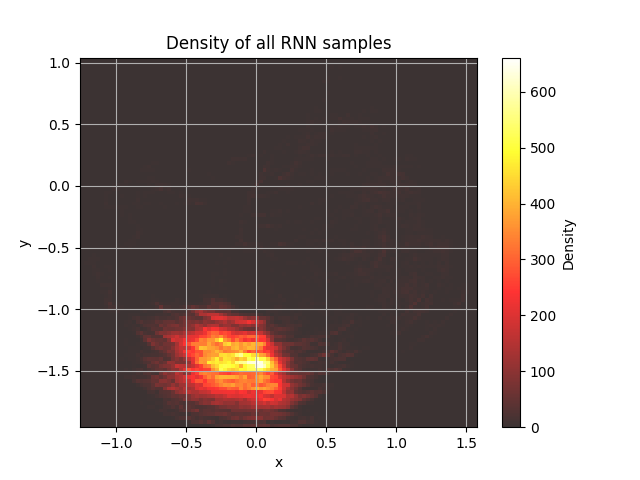
\includegraphics[scale=0.4]{RNN_density.png}
        \caption{A heat map of pendulum 2 in the predicted RNN model}
        \label{figRNND}
    \end{minipage}\hfill
    \begin{minipage}{0.48\textwidth}
        \centering
        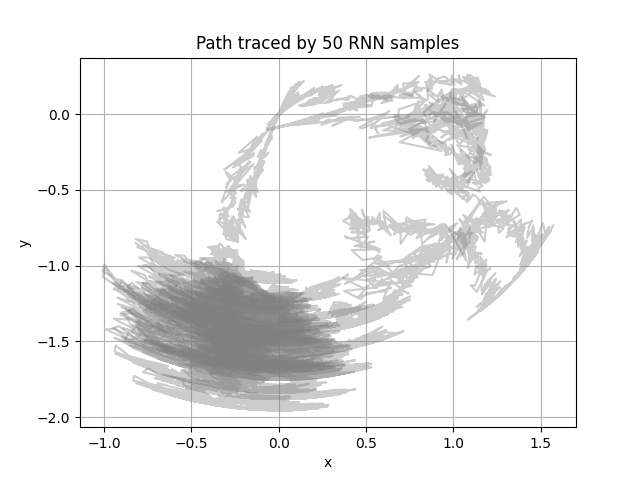
\includegraphics[scale=0.4]{RNN_50traced.png}
        \caption{50 samples of pendulum 2 traced with the RNN model}
        \label{figRNNT}
    \end{minipage}
    \caption{We see here better density than that of Fig [\ref{figNND}], but it seems like the model has misunderstood the oscillation, and has a bias towards going to the left. A similar story is told in the traced image. This suggests that the model has understood oscillation, but has somehow not understood where it should take place. Additionally, while the motion seems more controlled than Fig. [\ref{figNNT}], there are still a few massive outliers. \newline
    Notice also that the oscillation is much more concentrated. This suggests that the model should've had less emphasis put on samples "mid oscillation", that is, in the process of going left to right or opposite.}
    \label{figRNN}
\end{figure}
\newline
Lastly, let us look at CNN:
\begin{figure}[ht!]
    \centering
    
    \begin{minipage}{0.48\textwidth}
        \centering
        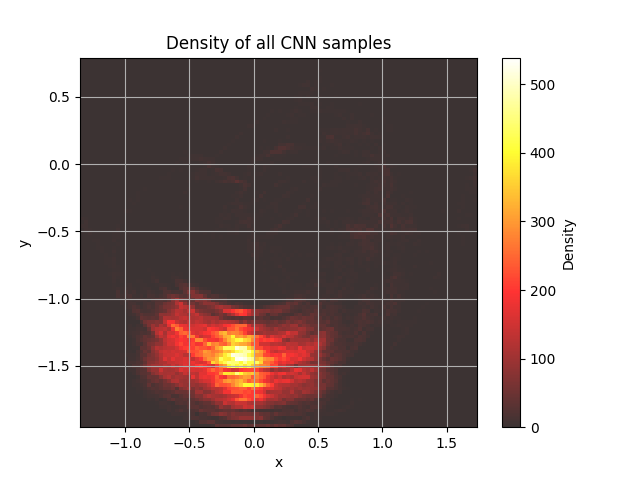
\includegraphics[scale=0.4]{CNN_density.png}
        \caption{A heat map of pendulum 2 in the predicted CNN model}
        \label{figRNND}
    \end{minipage}\hfill
    \begin{minipage}{0.48\textwidth}
        \centering
        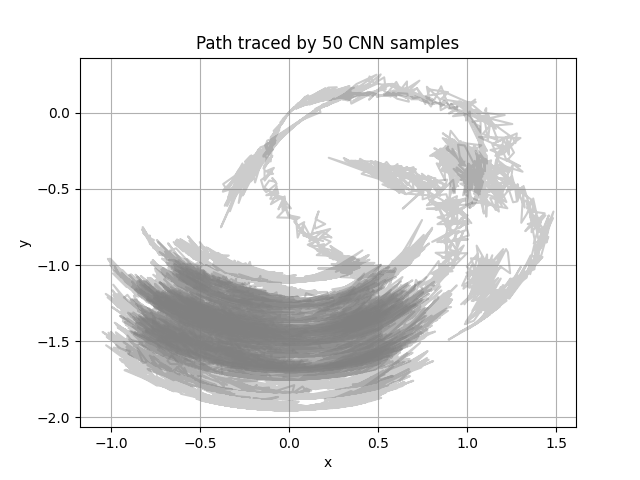
\includegraphics[scale=0.4]{CNN_50traced.png}
        \caption{50 samples of pendulum 2 traced with the CNN model}
        \label{figRNNT}
    \end{minipage}
    \caption{Here we see much the same behavior as in RNN, but the oscillating motion is better and less concentrated. It still has the outliers where it'll randomly shoot out.}
    \label{figCNN}
\end{figure}
\section{Discussion}
\subsection{Overfitting and underfitting}
It is hard to say specifically if overfitting or underfitting was the issue here. While the models managed to learn some of oscillating motion of the double pendulum system, it was still not "good enough" to be able to say that it could clearly model a double pendulum system. An other issue that can easy arise in cases like this that is quite hard to account for is that when splitting between train and test data, the majority of the test data were samples where the angles $\theta_1$, $\theta_2$ where initialized with negative values. This leads to a bias towards "left-side systems" and also increased the loss experienced when predicting the remaining "right-side systems". There is no easy way to fix this. Had it only been that the angles $\theta_1$ and $\theta_2$ that were randomized, we could've made it so both train and test had an even split, but this was not possible as all the other variables are also randomized (and could thus lead to similar biases). Perhaps evenly splitting $\theta_1$, $\theta_2$ in between train and test would've been the lesser of two evils.
\subsection{Numerical Stability and volatility of initial variables}
One of the inherent problems when generating data of a chaotic system like double pendulums is the numerical stability. Doubly so as we're dealing with randomized (within boundaries) initial conditions. This in turn means that we have to be careful when initializing the system. While this can be partially remedied by weeding out bad runs automatically, we still have a limited range of initial variables we can study. One of the key strengths of Neural Networks is that they can model for initial conditions they haven't seen before, and while that still remains true here, the limited number of initial variations does hurt this aspect of Neural Networks a bit.
\subsection{Parallelization}
One of the strongest cases and what could probably be done to further improve or expand upon this project is to implement some kind of parallel programming. Whereas traditional numerical methods like the RK4 is reliant on a previous data point to make predictions, thus making them cumbersome to parallelize, NNs are immune to this issue. As long as the model is trained, an infinite (theoretically) number of predictions can be run in parallel.
\newpage
\subsection{Further improvements - Unimplemented methods}
There are two sections of the code that are left in despite not working and ultimately going unused. Firstly, a grid-search algorithm that intends to find the best possible hyper-parameters, activation functions, learning rates etc. This ultimately did not work, sadly, which does mean more time has to be spent manually checking possible combinations and their associated models/losses. This is doubly cumbersome for RNN and CNN which both take a fairly long time to train. \newline
Secondly is a custom loss function. While the losses seem fine with a normal loss function implementation (in this case MSE), these are somewhat deceptive. When using the function \texttt{plot\textunderscore random \textunderscore sample()} we see that, despite very low losses, the predicted model doesn't look much like the real thing at all. Alternatively, these can be viewed \href{https://github.com/simloken/FYS5429/blob/main/Project/figures/randomly_sampled_run_NN.gif}{here}, \href{https://github.com/simloken/FYS5429/blob/main/Project/figures/randomly_sampled_run_RNN.gif}{here} and \href{https://github.com/simloken/FYS5429/blob/main/Project/figures/randomly_sampled_run_CNN.gif}{here} for NN, RNN and CNN respectively. The idea was that, assuming there is zero loss of energy in the system, we could take the initial energy of the system at $t=0$, and use that as an upper limit to the energy. Thus, if at any point the energy of the system went beyond that, the model would be penalized. This in turn \emph{should} have made for a better model, but ultimately ended up not working. This would probably also solved the most prevalent issue in the RNN and CNN model, with the random jittery movement where the second pendulum shoots out of the oscillating motion.
\section{Conclusion}
In closing, we've shown how to create a chaotic double pendulum system and use that system to generate data that we can then use to train different Neural Networks and weigh them against each other. We've also seen how the different models handle predicting the motion of double pendulums and how some models perform better than others. Ultimately, it is hard to draw a conclusion as to which model best predicts the chaotic motion of double pendulums, but a strong case can be made for CNNs, especially if we could "clamp" the energy of the system.
\bibliographystyle{plainurl}
\bibliography{citations.bib}
\newpage
\renewcommand*\appendixpagename{\Large Appendices}
\appendixpage
\addappheadtotoc
\renewcommand{\thesubsection}{\Alph{subsection}}
\subsection{Appendix Title}
\subsubsection{Code}
Any code can be found at my \href{https://github.com/simloken/FYS5429/tree/main/Project}{github}
\end{document}
